\chapter{Background}
\label{sec:demo}
%
In this chapter bla bla

% ====
% Autonomic computing
% ====
\section{Autonomic computing}
Autonomic computing is an architecture for computing systems to enable the ability to manage themselves in accordance to high level objectives configured by administrators \cite{Kephart2003VisionComputing}. 
These computing systems dynamically adapt to demands and conditions of the workload \cite{Kephart2003VisionComputing}.
An intelligent control-loop is responsible to collect all important details of the computing system and make decision according to the collected details. To automate the tasks, the intelligent control-loop is organized into four categories:

\begin{itemize}
\item \textbf{Self-configuring}
- Components in the environment have to adapt dynamically to system changes using policies. For example, deploying or removing new components.

\item \textbf{Self-healing}
- If system errors have being detected, the control-loop has to perform policy-based actions without disrupting the 
environment.

\item \textbf{Self-optimizing}
- The control-loop has to monitor the resources and should adapt to changes dynamically.

\item \textbf{Self-protecting}
- Detection and protection against threats.

\end{itemize}

 An autonomic computing environment consists of an autonomic manager, managed-resources and a knowledge-base.
 % As shown in figure ...
 
\subsection{Managed resources}
Managed resources are software or hardware components in the computing environment. For example, a managed resource 
can be a database, service, application, server or different entity. Each managed resource implements an interface to enable 
the autonomic manager to communicate with the managed resource. 

These interface are called touchpoints.

\subsection{Autonomic manager}
The autonomic manager implements an intelligent control-loop to collect system metrics from the managed resources and acts according to the collected details. It can only make adjustments within it`s own scope and uses policies to make decisions of what actions have to be
executed to accommodate the objectives.
To be self-managing, the autonomic manager has to implement the following four automated functions.

\begin{itemize}
\item \textbf{Monitor}
- The monitor function is responsible to collect the needed metrics from all managed resources and applies aggregation and filter
operations to the collected data. After that the function reports the metrics.

\item \textbf{Analyze}
- To determine if changes have to be made to the computing system, the collected data has to be analyzed.

\item \textbf{Plan}
- If changes have to be made, an appropriate change plan has to be generated. A change plan consists of actions that are needed to achieve the configured goals and objectives. The change plan needs to be forwarded to the execute function.

\item \textbf{Execute}
- The execute function applies all necessary changes to the computing system.

\end{itemize}

Multiple autonomic manager can exist in an autonomic computing environment to perform only certain parts. For example, 
there can be one autonomic manager which is responsible to monitor and analyze the system and another autonomic manager 
to plan and execute. To create a complete and closed control-loop, multiple autonomic manager can be composed together.


\section{Docker}


\section{Apache Spark}
Apache Spark is an open-source computing framework for parallel data processing on a large computer cluster. Spark manages the available resources and distributes computation tasks across a cluster to perform big-data processing operations at large scale \cite{Chambers2018Spark}. Before Spark was developed, Hadoop MapReduce \cite{Dean2010MapReduce} was the framework of choice for parallel operations on a computer cluster \cite{Zaharia2010Spark}. Spark accomplished to outperform Hadoop by 10x for iterative Machine Learning \cite{Zaharia2010Spark}. It is implemented in Scala\footnote{Scala programming language. https://www.scala-lang.org/}, a JVM-based language and provides a programming interface for Scala, Java\footnote{Java programming language. https://www.oracle.com/java/}, Python\footnote{Python programming language. https://www.python.org/} and R\footnote{R programming language. https://www.r-project.org/}. In addition, Spark includes an interactive SQL shell and libraries to implement Machine Learning and streaming applications \cite{Chambers2018Spark}.
It was developed in 2009 as the Spark research project at UC Berkeley and became an Apache Software Foundation project in 2013 \cite{Chambers2018Spark}. 

%  MASTER SLAVE 

\subsection{Spark programming model}

Spark provides resilient distributed datasets (RDDs) as the main abstractation for parallel operations \cite{Zaharia2010Spark}. Core types of Spark`s higher-level structured API are built on top of RDDs \cite{Chambers2018Spark} and will automatically be optimized by Spark`s Catalyst optimizer to run operations quick and efficient \cite{Hien2018Spark}.

\paragraph{Resilient distributed datasets:}
% What are RDDs
Resilient distributed datasets are fault-tolerant, parallel data structures to enable data sharing across cluster applications \cite{Zaharia2012RDDs}. They allow to express different cluster programming models like MapReduce, SQL and batched stream processing \cite{Zaharia2012RDDs}. RDDs have been implemented in Spark and serve as the underlying data structure for higher level APIs (Spark structured API) \cite{Zaharia2012RDDs}.
% How can RDDs be used in applications    !! HIER MAL BEISPIEL WIE IN RDD ERZEUGT WIRD
RDD`s are a immutable, partitioned collection of records and can only be initiated through transformations (e.g. map, filter) on data or other RDD`s.
% What are the advantages of RDDs    !!! HIER NOCHMAL BEISPIEL WIE DAS AUSSEHEN KANN
An advantage of RDDs is, that they can be recovered through lineage. Lost partitions of an RDD can be recomputed from other RDDs in parallel on different nodes \cite{Zaharia2012RDDs}. 
% Better use structured API
RDDs are lower level APIs and should only be used in applications if custom data partitioning is needed \cite{Chambers2018Spark}. It is recommended to use Sparks structured API objects instead. Optimizations for RDDs have to be implemented manually while Spark automatically optimize the execution for structured API operations \cite{Chambers2018Spark}.


\paragraph{Spark structured API:}
% What is the structured API
Spark provides high level structured APIs for manipulating all kinds of data. The three distributed core types are Datasets, DataFrames and SQL Tables and Views \cite{Chambers2018Spark}.
% About DataFrames, Datasets and SQL
Datasets and DataFrames are immutable, lazy evaluated collections that provide execution plans for operations \cite{Chambers2018Spark}. SQL Tables and Views work the same way as DataFrames, except that SQL is used as the interface instead of using the DataFrame programming interface \cite{Chambers2018Spark}.
% Differences between Datasets ad Dataframes
Datasets use JVM types and are therefore only available for JVM based languages. DataFrames are Datasets of type Row, which is the Spark internal optimized format for computations. This has advantages over JVM types which comes with garbage collection and object instantiation \cite{Chambers2018Spark}.


\paragraph{Spark Catalyst:}
% What is the Catalyst optimizer
Spark also provides a query optimizer engine called Spark Catalyst. The Spark Catalyst optimizer automatically optimizes Spark applications to run quickly and efficient.
% Short How
Before executing the user`s code, the Catalyst optimizer translates the data-processing logic into a logical plan and optimizes the plan using heuristics \cite{Hien2018Spark}. After that, the Catalyst optimizer converts the logical plan into a physical plan to create code that can be executed \cite{Hien2018Spark}.


% What are logical plans
Logical plans get created from a DataFrame or a SQL query. A logical plan represents the data-processing logic as a tree of operators and expressions where the Catalyst optimizer can apply sets of rule-based and cost-based optimizations \cite{Hien2018Spark}.
For example, the Catalyst can position a filter transformation in front of a join operation \cite{Hien2018Spark}.

% What are physical plans
From the logical plan, the Catalyst optimizer creates one ore more physical plans. The cheapest physical will be generated into Java bytecode for execution \cite{Hien2018Spark}.

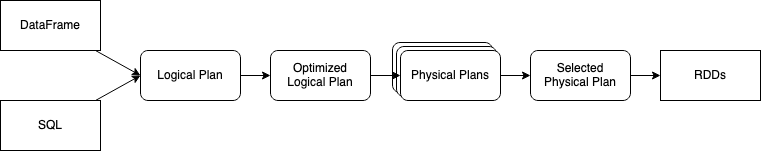
\includegraphics[scale=1]{images/03_background/spark_catalyst.png}


\paragraph{Structured API execution}
% Short Introduction

% How logical plans are created

% How physical plans are created


\subsection{Cluster modes}

\subsection{Spark application implementation}


\section{Prometheus}


\section{NVIDIA RAPIDS}


\section{Gitlab CI/CD}


\section{K-MEANS}


\section{Naive Bayes Classifier}
